\batchmode


\documentclass{article}
\RequirePackage{ifthen}


\usepackage{html,makeidx,epsf}
\usepackage{graphicx}
\usepackage{amssymb}
\usepackage{amsmath}
\usepackage[overload]{empheq}


\htmladdtonavigation{\htmladdnormallink
  {\htmladdimg{jetscalecropped.png}}{cv.pdf}}


\makeindex




\usepackage{xcolor}

\usepackage[]{inputenc}



\makeatletter

\makeatletter
\count@=\the\catcode`\_ \catcode`\_=8 
\newenvironment{tex2html_wrap}{}{}%
\catcode`\<=12\catcode`\_=\count@
\newcommand{\providedcommand}[1]{\expandafter\providecommand\csname #1\endcsname}%
\newcommand{\renewedcommand}[1]{\expandafter\providecommand\csname #1\endcsname{}%
  \expandafter\renewcommand\csname #1\endcsname}%
\newcommand{\newedenvironment}[1]{\newenvironment{#1}{}{}\renewenvironment{#1}}%
\let\newedcommand\renewedcommand
\let\renewedenvironment\newedenvironment
\makeatother
\let\mathon=$
\let\mathoff=$
\ifx\AtBeginDocument\undefined \newcommand{\AtBeginDocument}[1]{}\fi
\newbox\sizebox
\setlength{\hoffset}{0pt}\setlength{\voffset}{0pt}
\addtolength{\textheight}{\footskip}\setlength{\footskip}{0pt}
\addtolength{\textheight}{\topmargin}\setlength{\topmargin}{0pt}
\addtolength{\textheight}{\headheight}\setlength{\headheight}{0pt}
\addtolength{\textheight}{\headsep}\setlength{\headsep}{0pt}
\setlength{\textwidth}{349pt}
\newwrite\lthtmlwrite
\makeatletter
\let\realnormalsize=\normalsize
\global\topskip=2sp
\def\preveqno{}\let\real@float=\@float \let\realend@float=\end@float
\def\@float{\let\@savefreelist\@freelist\real@float}
\def\liih@math{\ifmmode$\else\bad@math\fi}
\def\end@float{\realend@float\global\let\@freelist\@savefreelist}
\let\real@dbflt=\@dbflt \let\end@dblfloat=\end@float
\let\@largefloatcheck=\relax
\let\if@boxedmulticols=\iftrue
\def\@dbflt{\let\@savefreelist\@freelist\real@dbflt}
\def\adjustnormalsize{\def\normalsize{\mathsurround=0pt \realnormalsize
 \parindent=0pt\abovedisplayskip=0pt\belowdisplayskip=0pt}%
 \def\phantompar{\csname par\endcsname}\normalsize}%
\def\lthtmltypeout#1{{\let\protect\string \immediate\write\lthtmlwrite{#1}}}%
\usepackage[tightpage,active]{preview}
\newbox\lthtmlPageBox
\newdimen\lthtmlCropMarkHeight
\newdimen\lthtmlCropMarkDepth
\long\def\lthtmlTightVBox#1#2{%
    \setbox\lthtmlPageBox\vbox{\hbox{\catcode`\_=8 #2}}%
    \lthtmlCropMarkHeight=\ht\lthtmlPageBox \advance \lthtmlCropMarkHeight 6pt
    \lthtmlCropMarkDepth=\dp\lthtmlPageBox
    \lthtmltypeout{^^J:#1:lthtmlCropMarkHeight:=\the\lthtmlCropMarkHeight}%
    \lthtmltypeout{^^J:#1:lthtmlCropMarkDepth:=\the\lthtmlCropMarkDepth:1ex:=\the \dimexpr 1ex}%
    \begin{preview}\copy\lthtmlPageBox\end{preview}}%
\long\def\lthtmlTightFBox#1#2{%
    \adjustnormalsize\setbox\lthtmlPageBox=\vbox\bgroup %
    \let\ifinner=\iffalse \let\)\liih@math %
    {\catcode`\_=8 #2}%
    \@next\next\@currlist{}{\def\next{\voidb@x}}%
    \expandafter\box\next\egroup %
    \lthtmlCropMarkHeight=\ht\lthtmlPageBox \advance \lthtmlCropMarkHeight 6pt
    \lthtmlCropMarkDepth=\dp\lthtmlPageBox
    \lthtmltypeout{^^J:#1:lthtmlCropMarkHeight:=\the\lthtmlCropMarkHeight}%
    \lthtmltypeout{^^J:#1:lthtmlCropMarkDepth:=\the\lthtmlCropMarkDepth:1ex:=\the \dimexpr 1ex}%
    \begin{preview}\copy\lthtmlPageBox\end{preview}}%
    \long\def\lthtmlinlinemathA#1#2\lthtmlindisplaymathZ{\lthtmlTightVBox{#1}{#2}}
    \def\lthtmlinlineA#1#2\lthtmlinlineZ{\lthtmlTightVBox{#1}{#2}}
    \long\def\lthtmldisplayA#1#2\lthtmldisplayZ{\lthtmlTightVBox{#1}{#2}}
    \long\def\lthtmlinlinemathA#1#2\lthtmlindisplaymathZ{\lthtmlTightVBox{#1}{#2}}
    \def\lthtmlinlineA#1#2\lthtmlinlineZ{\lthtmlTightVBox{#1}{#2}}
    \long\def\lthtmldisplayA#1#2\lthtmldisplayZ{\lthtmlTightVBox{#1}{#2}}
    \long\def\lthtmldisplayB#1#2\lthtmldisplayZ{\\edef\preveqno{(\theequation)}%
        \lthtmlTightVBox{#1}{\let\@eqnnum\relax#2}}
    \long\def\lthtmlfigureA#1#2\lthtmlfigureZ{\let\@savefreelist\@freelist
        \lthtmlTightFBox{#1}{#2}\global\let\@freelist\@savefreelist}
    \long\def\lthtmlpictureA#1#2\lthtmlpictureZ{\let\@savefreelist\@freelist
        \lthtmlTightVBox{#1}{#2}\global\let\@freelist\@savefreelist}
\def\lthtmlcheckvsize{\ifdim\ht\sizebox<\vsize 
  \ifdim\wd\sizebox<\hsize\expandafter\hfill\fi \expandafter\vfill
  \else\expandafter\vss\fi}%
\providecommand{\selectlanguage}[1]{}%
\makeatletter \tracingstats = 1 
\providecommand{\Tau}{\textrm{T}}
\providecommand{\Chi}{\textrm{X}}
\providecommand{\Zeta}{\textrm{Z}}
\providecommand{\Beta}{\textrm{B}}
\providecommand{\Omicron}{\textrm{O}}
\providecommand{\Epsilon}{\textrm{E}}
\providecommand{\Nu}{\textrm{N}}
\providecommand{\Alpha}{\textrm{A}}
\providecommand{\omicron}{\textrm{o}}
\providecommand{\Iota}{\textrm{J}}
\providecommand{\Mu}{\textrm{M}}
\providecommand{\Kappa}{\textrm{K}}
\providecommand{\Rho}{\textrm{R}}
\providecommand{\Eta}{\textrm{H}}


\begin{document}
\pagestyle{empty}\thispagestyle{empty}\lthtmltypeout{}%
\lthtmltypeout{latex2htmlLength hsize=\the\hsize}\lthtmltypeout{}%
\lthtmltypeout{latex2htmlLength vsize=\the\vsize}\lthtmltypeout{}%
\lthtmltypeout{latex2htmlLength hoffset=\the\hoffset}\lthtmltypeout{}%
\lthtmltypeout{latex2htmlLength voffset=\the\voffset}\lthtmltypeout{}%
\lthtmltypeout{latex2htmlLength topmargin=\the\topmargin}\lthtmltypeout{}%
\lthtmltypeout{latex2htmlLength topskip=\the\topskip}\lthtmltypeout{}%
\lthtmltypeout{latex2htmlLength headheight=\the\headheight}\lthtmltypeout{}%
\lthtmltypeout{latex2htmlLength headsep=\the\headsep}\lthtmltypeout{}%
\lthtmltypeout{latex2htmlLength parskip=\the\parskip}\lthtmltypeout{}%
\lthtmltypeout{latex2htmlLength oddsidemargin=\the\oddsidemargin}\lthtmltypeout{}%
\makeatletter
\if@twoside\lthtmltypeout{latex2htmlLength evensidemargin=\the\evensidemargin}%
\else\lthtmltypeout{latex2htmlLength evensidemargin=\the\oddsidemargin}\fi%
\lthtmltypeout{}%
\makeatother
\setcounter{page}{1}
\onecolumn

% !!! IMAGES START HERE !!!

{\newpage\clearpage
\lthtmlinlinemathA{tex2html_wrap_inline1974}%
$ 10000$%
\lthtmlindisplaymathZ
\lthtmlcheckvsize\clearpage}

{\newpage\clearpage
\lthtmlinlinemathA{tex2html_wrap_inline1978}%
$ \qopname  \relax o{cos}(20 \pi t) + \qopname  \relax o{sin}(2 \pi t)$%
\lthtmlindisplaymathZ
\lthtmlcheckvsize\clearpage}

\stepcounter{section}
{\newpage\clearpage
\lthtmlinlinemathA{tex2html_wrap_inline1981}%
$\textstyle \parbox{\textwidth}{
\par
I graduated in 2009 from Munkkiniemi high school. Mathematics was a subject I had naturally thrived in -- so, after some bumps and turns,  I found myself at the University of Helsinki studying mathematics. And yeah, indeed, I love mathematics -- I love the apparent universality of it. This subject is without a doubt debatable, but, at least in some sense, I like to think that mathematical truths are universal in the truest sense of the word; they are eternal, they are the same everywhere, regardless of the physical universe we live in. Alien in another galaxy will end up in the same mathematical truths we do. Alien in another universe will end up in the same mathematical truths we do. Mathematics has the power to explain what we see in our everyday life. Mathematics is not only natural science but a form of art and poetry. Mathematics is music -- music is mathematics.
\par
While studying mathematics, physics and computer science, I took some courses on economics. That inspired me to write my bachelor's thesis on optimal control theory. I worked on the problem of how increasing public investments affects the GDP. I did not find any breakthrough, but it was an intriguing subject.
\par
I proceeded with my graduate studies studying applied mathematics. I studied subjects like partial differential equations, functional analysis, dynamical systems, and  -- the University of Helsinki's proudness -- complex analysis. (My thesis advisor said that, in a moral sense, you cannot graduate from the University of Helsinki without taking some courses on Complex analysis, because a lot of the discipline has been developed in the university.) In addition, as a more ``practical'' subject, I studied some inverse problems. Summa summarum, I studied a wide range of fields in mathematics.
\par
During my graduate studies, I spent half a year in Utrecht, Netherlands, studying more applied analysis of varying subjects (searching periodic orbits in the Lorentz attractor as an example of a course -- that I failed). At Utrecht University, I got the inspiration for a subject for my future master's thesis; the Finite Element Method. After I got back to Helsinki from the exchange, I had a chance to study more about the finite element method in Aalto University's courses. (Aalto University is a consortium of the Helsinki University of Technology, the Helsinki School of Economics and the University of Art and Design Helsinki.) While writing my thesis I also taught basic mathematics courses at the University of Helsinki and gained valuable experience in the pedagogical area.
\par
In the binge of graduation, I started to look for future opportunities. I looked for coding jobs in Helsinki and Tallinn, jobs for mathematicians in the mapping industry, continuing at some universities to pursue a PhD etc. I am glad I had the chance to use my creativity and continue in Aalto University's Department of Signal Processing and Acoustics to research low earth orbit satellite communications. The research methodology was from a stochastic geometry perspective, that was well aligned with my mathematical background.
\par
My professional ambitions are in improving the lives of people globally. Communications play an essential in the picture. (But contain some challenging problems also, as we have seen with the social media.) Through effective communication, we can share knowledge, control resources, discuss issues etc. -- however, globally, the communication infrastructure is still not nearly complete. My interests contain, but are not limited to, communications, particularly wireless networks and signal processing. My dream is to share my knowledge in the process toward a free and honest world. (Pardon me for the cliches.)
\par
}$%
\lthtmlindisplaymathZ
\lthtmlcheckvsize\clearpage}

\stepcounter{subsection}
\stepcounter{subsection}
\stepcounter{subsection}
\stepcounter{section}
\stepcounter{subsection}
{\newpage\clearpage
\lthtmlinlinemathA{tex2html_wrap_inline1991}%
$ A = [-\pi,\pi] \times [-1,1]$%
\lthtmlindisplaymathZ
\lthtmlcheckvsize\clearpage}

{\newpage\clearpage
\lthtmlinlinemathA{tex2html_wrap_inline1993}%
$ A$%
\lthtmlindisplaymathZ
\lthtmlcheckvsize\clearpage}

{\newpage\clearpage
\lthtmlinlinemathA{tex2html_wrap_indisplay1995}%
$\displaystyle (x,y) \mapsto (1,x,\sin^{-1}(y)) .$%
\lthtmlindisplaymathZ
\lthtmlcheckvsize\clearpage}

{\newpage\clearpage
\lthtmlinlinemathA{tex2html_wrap_inline1997}%
$ (r,\theta,\varphi)$%
\lthtmlindisplaymathZ
\lthtmlcheckvsize\clearpage}

{\newpage\clearpage
\lthtmlinlinemathA{tex2html_wrap_inline1999}%
$ r$%
\lthtmlindisplaymathZ
\lthtmlcheckvsize\clearpage}

\stepcounter{subsection}
\stepcounter{subsection}
\stepcounter{subsection}
\stepcounter{subsection}
\stepcounter{subsection}
{\newpage\clearpage
\lthtmlinlinemathA{tex2html_wrap_indisplay2021}%
$\displaystyle \textbf{P}[$%
\lthtmlindisplaymathZ
\lthtmlcheckvsize\clearpage}

{\newpage\clearpage
\lthtmlinlinemathA{tex2html_wrap_indisplay2022}%
$\displaystyle ] = e^{-\frac{\pi^2}{2\sqrt{P}}},$%
\lthtmlindisplaymathZ
\lthtmlcheckvsize\clearpage}

{\newpage\clearpage
\lthtmlinlinemathA{tex2html_wrap_inline2024}%
$ P$%
\lthtmlindisplaymathZ
\lthtmlcheckvsize\clearpage}

{\newpage\clearpage
\lthtmlinlinemathA{tex2html_wrap_inline2026}%
$ (1)$%
\lthtmlindisplaymathZ
\lthtmlcheckvsize\clearpage}

{\newpage\clearpage
\lthtmlinlinemathA{tex2html_wrap_indisplay2029}%
$\displaystyle ]  = 1-\left(1-e^{-\frac{\pi^2}{2\sqrt{P/N}}}\right)^N,$%
\lthtmlindisplaymathZ
\lthtmlcheckvsize\clearpage}

{\newpage\clearpage
\lthtmlinlinemathA{tex2html_wrap_inline2031}%
$ N$%
\lthtmlindisplaymathZ
\lthtmlcheckvsize\clearpage}

\stepcounter{subsection}
\stepcounter{subsection}
\stepcounter{subsection}
{\newpage\clearpage
\lthtmlinlinemathA{tex2html_wrap_inline2052}%
$ [0, \infty)$%
\lthtmlindisplaymathZ
\lthtmlcheckvsize\clearpage}

{\newpage\clearpage
\lthtmlinlinemathA{tex2html_wrap_inline2054}%
$ Y_j$%
\lthtmlindisplaymathZ
\lthtmlcheckvsize\clearpage}

{\newpage\clearpage
\lthtmlinlinemathA{tex2html_wrap_inline2056}%
$ B(r_1,r_2)$%
\lthtmlindisplaymathZ
\lthtmlcheckvsize\clearpage}

{\newpage\clearpage
\lthtmlinlinemathA{tex2html_wrap_inline2058}%
$ 2\int_{r_1}^{r^2} \frac{1}{\sqrt{2 \pi}}e^{-y^2} dy.$%
\lthtmlindisplaymathZ
\lthtmlcheckvsize\clearpage}

{\newpage\clearpage
\lthtmlinlinemathA{tex2html_wrap_indisplay2059}%
$\displaystyle \mathcal{L}_{\tau}(f)$%
\lthtmlindisplaymathZ
\lthtmlcheckvsize\clearpage}

{\newpage\clearpage
\lthtmlinlinemathA{tex2html_wrap_indisplay2060}%
$\displaystyle = \mathbb{E} \exp \left[-\sum_i f(|Y_i|) \right] = \mathbb{E}  \prod_i \exp \left[  -f(|Y_i|)   \right]$%
\lthtmlindisplaymathZ
\lthtmlcheckvsize\clearpage}

{\newpage\clearpage
\lthtmlinlinemathA{tex2html_wrap_indisplay2061}%
$\displaystyle = \mathbb{E}_n \left[  (2 \pi)^{-n/2}  \int_0^{\infty} \dots \int_0^{\infty}  \prod_{i = 0}^n \exp \left[  -f(y_i)  \right] \frac{2}{\sqrt{2 \pi}}e^{-y_i^2} dy_1 \dots d y_n \right]$%
\lthtmlindisplaymathZ
\lthtmlcheckvsize\clearpage}

{\newpage\clearpage
\lthtmlinlinemathA{tex2html_wrap_indisplay2062}%
$\displaystyle = \mathbb{E}_n \left[(2 \pi)^{-n/2}  \left( \int_{0}^{\infty}  2\exp \left[  -f(y) - y^2   \right] dy \right)^n\right]$%
\lthtmlindisplaymathZ
\lthtmlcheckvsize\clearpage}

{\newpage\clearpage
\lthtmlinlinemathA{tex2html_wrap_indisplay2063}%
$\displaystyle = \mathbb{E}_n \exp \left[ \sum_{i= 0}^n \log \left(   \int_{0}^{\infty}  \exp \left[  -f(y)  \right] \frac{2e^{-y^2}}{\sqrt{2 \pi}} dy \right) \right]$%
\lthtmlindisplaymathZ
\lthtmlcheckvsize\clearpage}

{\newpage\clearpage
\lthtmlinlinemathA{tex2html_wrap_inline2065}%
$ \mathcal{L}(g)$%
\lthtmlindisplaymathZ
\lthtmlcheckvsize\clearpage}

{\newpage\clearpage
\lthtmlinlinemathA{tex2html_wrap_inline2067}%
$ g = - \log \left(   \int_{0}^{\infty}  \exp \left[  -f(y)  \right] \frac{e^{-y^2}}{\sqrt{2 \pi}} dy \right)  $%
\lthtmlindisplaymathZ
\lthtmlcheckvsize\clearpage}

{\newpage\clearpage
\lthtmlinlinemathA{tex2html_wrap_indisplay2068}%
$\displaystyle \mathcal{L}(g) = \mathcal{L}_{\tau}(f)$%
\lthtmlindisplaymathZ
\lthtmlcheckvsize\clearpage}

{\newpage\clearpage
\lthtmlinlinemathA{tex2html_wrap_indisplay2069}%
$\displaystyle = \exp \left[  -\int_{\mathbb{R}^2} 1 -  e^{\log \left(   \int_{0}^{\infty}  \exp \left[  -f(y)   \right] \frac{2e^{-y^2}}{\sqrt{2 \pi}} dy \right) }\Lambda(dx) \right]$%
\lthtmlindisplaymathZ
\lthtmlcheckvsize\clearpage}

{\newpage\clearpage
\lthtmlinlinemathA{tex2html_wrap_indisplay2070}%
$\displaystyle = \exp \left[-\int_{\mathbb{R}^2} \left(1  -   \int_{0}^{\infty}  \exp [-f(y)] \frac{2e^{-y^2}}{\sqrt{2 \pi}}  dy \right)  \Lambda(dx)  \right]$%
\lthtmlindisplaymathZ
\lthtmlcheckvsize\clearpage}

{\newpage\clearpage
\lthtmlinlinemathA{tex2html_wrap_indisplay2071}%
$\displaystyle = \exp \left[-\int_{\mathbb{R}^2}\int_{0}^{\infty} \left(1  -     \exp [-f(y)]   \right) \frac{2e^{-y^2}}{\sqrt{2 \pi}}dy  \Lambda(dx)  \right]$%
\lthtmlindisplaymathZ
\lthtmlcheckvsize\clearpage}

{\newpage\clearpage
\lthtmlinlinemathA{tex2html_wrap_indisplay2072}%
$\displaystyle = \exp \left[-\int_{0}^{\infty} \left(1  -     \exp [-f(y)]   \right)  \sqrt{\frac{2}{\pi}}e^{-y^2} N dy    \right], (1)$%
\lthtmlindisplaymathZ
\lthtmlcheckvsize\clearpage}

{\newpage\clearpage
\lthtmlinlinemathA{tex2html_wrap_inline2080}%
$ \sqrt{\frac{2}{\pi}}e^{-x^2} N.$%
\lthtmlindisplaymathZ
\lthtmlcheckvsize\clearpage}

{\newpage\clearpage
\lthtmlpictureA{tex2html_wrap2088}%
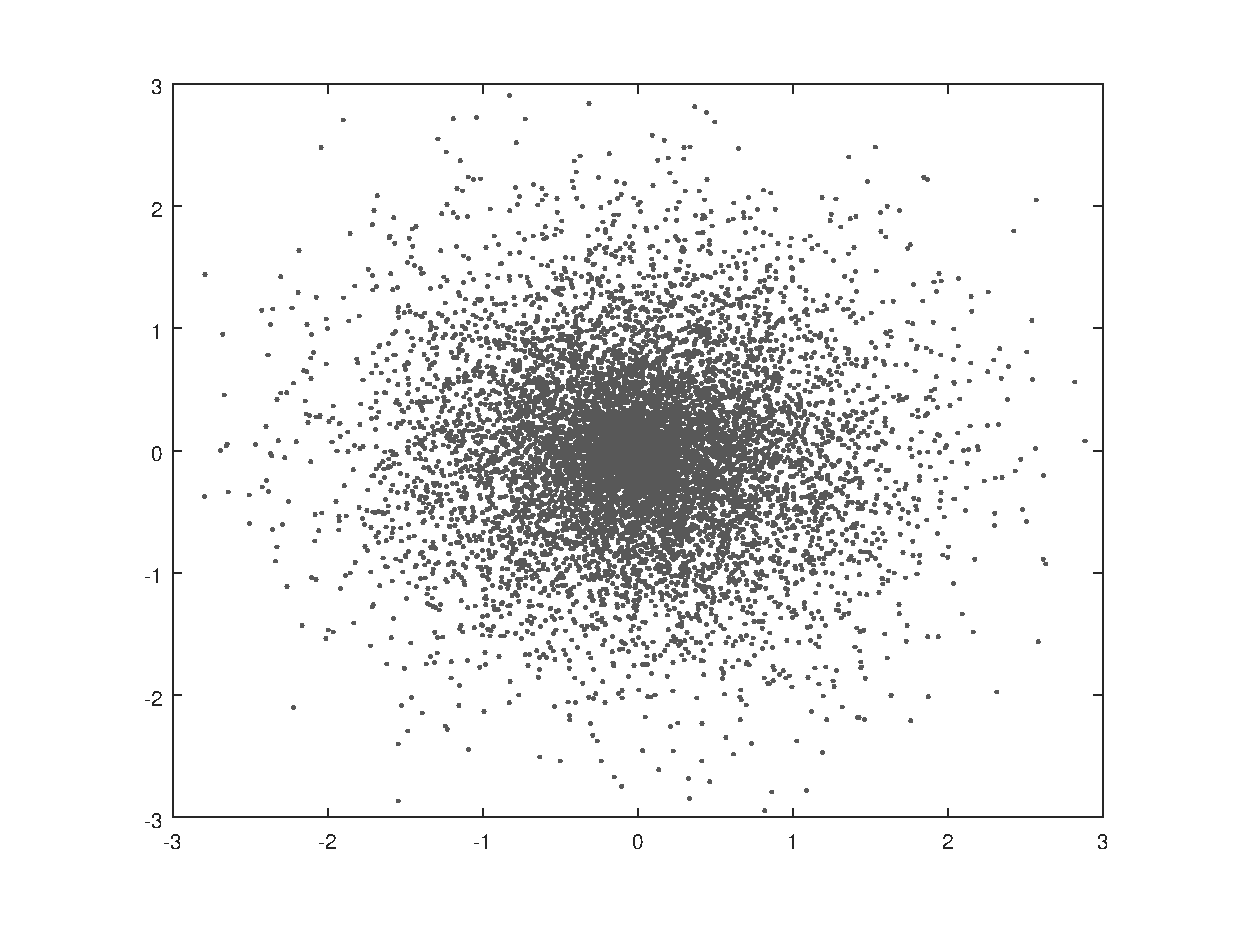
\includegraphics[width=\linewidth]{spread.eps}%
\lthtmlpictureZ
\lthtmlcheckvsize\clearpage}

\stepcounter{subsection}
{\newpage\clearpage
\lthtmlinlinemathA{tex2html_wrap_inline2091}%
$ F_s$%
\lthtmlindisplaymathZ
\lthtmlcheckvsize\clearpage}

{\newpage\clearpage
\lthtmlinlinemathA{tex2html_wrap_inline2093}%
$ F_s/2$%
\lthtmlindisplaymathZ
\lthtmlcheckvsize\clearpage}

\stepcounter{subsection}
{\newpage\clearpage
\lthtmlinlinemathA{tex2html_wrap_inline2096}%
$ S(t)$%
\lthtmlindisplaymathZ
\lthtmlcheckvsize\clearpage}

{\newpage\clearpage
\lthtmlinlinemathA{tex2html_wrap_inline2098}%
$ t \mapsto \frac{\sin(2 \pi B_L t)}{\pi t}$%
\lthtmlindisplaymathZ
\lthtmlcheckvsize\clearpage}

{\newpage\clearpage
\lthtmlinlinemathA{tex2html_wrap_inline2102}%
$ B_L$%
\lthtmlindisplaymathZ
\lthtmlcheckvsize\clearpage}

{\newpage\clearpage
\lthtmlinlinemathA{tex2html_wrap_inline2104}%
$ t \mapsto \delta(t) -  \frac{\sin(2 \pi B_H t)}{\pi t},$%
\lthtmlindisplaymathZ
\lthtmlcheckvsize\clearpage}

{\newpage\clearpage
\lthtmlinlinemathA{tex2html_wrap_inline2106}%
$ \delta(t)$%
\lthtmlindisplaymathZ
\lthtmlcheckvsize\clearpage}

{\newpage\clearpage
\lthtmlinlinemathA{tex2html_wrap_inline2108}%
$ B_H$%
\lthtmlindisplaymathZ
\lthtmlcheckvsize\clearpage}

{\newpage\clearpage
\lthtmlinlinemathA{tex2html_wrap_indisplay2110}%
$\displaystyle \mathbb{Z} \ni i \mapsto \frac{\sin(2 \pi \frac{B_L}{f_c} i)}{\pi i},
$%
\lthtmlindisplaymathZ
\lthtmlcheckvsize\clearpage}

{\newpage\clearpage
\lthtmlinlinemathA{tex2html_wrap_indisplay2112}%
$\displaystyle i \mapsto \delta[i] - \frac{\sin(2 \pi \frac{B_H}{f_c} i)}{\pi i},
$%
\lthtmlindisplaymathZ
\lthtmlcheckvsize\clearpage}

{\newpage\clearpage
\lthtmlinlinemathA{tex2html_wrap_inline2114}%
$ f_c$%
\lthtmlindisplaymathZ
\lthtmlcheckvsize\clearpage}

{\newpage\clearpage
\lthtmlinlinemathA{tex2html_wrap_inline2116}%
$ i \mapsto \delta[i] := \delta_{0i} $%
\lthtmlindisplaymathZ
\lthtmlcheckvsize\clearpage}

{\newpage\clearpage
\lthtmlinlinemathA{tex2html_wrap_inline2120}%
$ \cos(20 \pi t) + \sin(2 \pi t)$%
\lthtmlindisplaymathZ
\lthtmlcheckvsize\clearpage}

\stepcounter{subsection}
{\newpage\clearpage
\lthtmlinlinemathA{tex2html_wrap_inline2129}%
$ (-2,10) \times(-10i, 10i) \subset \mathbb{C}.$%
\lthtmlindisplaymathZ
\lthtmlcheckvsize\clearpage}

{\newpage\clearpage
\lthtmlinlinemathA{tex2html_wrap_inline2131}%
$ \max = 2$%
\lthtmlindisplaymathZ
\lthtmlcheckvsize\clearpage}

{\newpage\clearpage
\lthtmlinlinemathA{tex2html_wrap_inline2135}%
$ 0.1$%
\lthtmlindisplaymathZ
\lthtmlcheckvsize\clearpage}

\stepcounter{section}
\stepcounter{subsection}
{\newpage\clearpage
\lthtmlinlinemathA{tex2html_wrap_inline2139}%
$ X \sim \mathcal{N}(\mu, \sigma^2)$%
\lthtmlindisplaymathZ
\lthtmlcheckvsize\clearpage}

{\newpage\clearpage
\lthtmlinlinemathA{tex2html_wrap_inline2141}%
$ X \approx Y \sim$%
\lthtmlindisplaymathZ
\lthtmlcheckvsize\clearpage}

{\newpage\clearpage
\lthtmlinlinemathA{tex2html_wrap_inline2142}%
$ (\mu_{\text{LN}}, \sigma_{\text{LN}}),$%
\lthtmlindisplaymathZ
\lthtmlcheckvsize\clearpage}

{\newpage\clearpage
\lthtmlinlinemathA{tex2html_wrap_indisplay2144}%
$\displaystyle \mu = \exp\left( \mu_{\text{LN}} + \frac{\sigma_{\text{LN}}^2}{2} \right)$%
\lthtmlindisplaymathZ
\lthtmlcheckvsize\clearpage}

{\newpage\clearpage
\lthtmlinlinemathA{tex2html_wrap_indisplay2146}%
$\displaystyle \sigma = (\exp( \sigma_{\text{LN}}^2) - 1)\exp(2 \mu_{\text{LN}} + \sigma_{\text{LN}}^2).$%
\lthtmlindisplaymathZ
\lthtmlcheckvsize\clearpage}

{\newpage\clearpage
\lthtmlinlinemathA{tex2html_wrap_inline2148}%
$ \mu_{\text{LN}}$%
\lthtmlindisplaymathZ
\lthtmlcheckvsize\clearpage}

{\newpage\clearpage
\lthtmlinlinemathA{tex2html_wrap_inline2150}%
$ \sigma_{\text{LN}}$%
\lthtmlindisplaymathZ
\lthtmlcheckvsize\clearpage}

{\newpage\clearpage
\lthtmlinlinemathA{tex2html_wrap_inline2152}%
$ X$%
\lthtmlindisplaymathZ
\lthtmlcheckvsize\clearpage}

{\newpage\clearpage
\lthtmlinlinemathA{tex2html_wrap_indisplay2154}%
$\displaystyle 1/X \approx 1/Y \sim$%
\lthtmlindisplaymathZ
\lthtmlcheckvsize\clearpage}

{\newpage\clearpage
\lthtmlinlinemathA{tex2html_wrap_indisplay2155}%
$\displaystyle (-\mu_{\text{LN}}, \sigma_{\text{LN}}).
$%
\lthtmlindisplaymathZ
\lthtmlcheckvsize\clearpage}

\stepcounter{subsection}
\stepcounter{subsection}
\stepcounter{subsection}
{\newpage\clearpage
\lthtmlinlinemathA{tex2html_wrap_inline2160}%
$ 2000$%
\lthtmlindisplaymathZ
\lthtmlcheckvsize\clearpage}

{\newpage\clearpage
\lthtmlinlinemathA{tex2html_wrap_inline2162}%
$ 35$%
\lthtmlindisplaymathZ
\lthtmlcheckvsize\clearpage}

{\newpage\clearpage
\lthtmlinlinemathA{tex2html_wrap_inline2164}%
$ 3$%
\lthtmlindisplaymathZ
\lthtmlcheckvsize\clearpage}

{\newpage\clearpage
\lthtmlinlinemathA{tex2html_wrap_inline2166}%
$ 1.5$%
\lthtmlindisplaymathZ
\lthtmlcheckvsize\clearpage}

\stepcounter{subsection}
{\newpage\clearpage
\lthtmlinlinemathA{tex2html_wrap_inline2169}%
$ t$%
\lthtmlindisplaymathZ
\lthtmlcheckvsize\clearpage}

{\newpage\clearpage
\lthtmlinlinemathA{tex2html_wrap_indisplay2171}%
$\displaystyle \{t \mapsto$%
\lthtmlindisplaymathZ
\lthtmlcheckvsize\clearpage}

{\newpage\clearpage
\lthtmlinlinemathA{tex2html_wrap_indisplay2172}%
$\displaystyle (F_s t - n)\}_n,
$%
\lthtmlindisplaymathZ
\lthtmlcheckvsize\clearpage}

{\newpage\clearpage
\lthtmlinlinemathA{tex2html_wrap_indisplay2178}%
$\displaystyle \{ x[n]\}_{n=0}^{N-1}
$%
\lthtmlindisplaymathZ
\lthtmlcheckvsize\clearpage}

{\newpage\clearpage
\lthtmlinlinemathA{tex2html_wrap_indisplay2180}%
$\displaystyle S(t) =\sum_{n = 0}^{N-1} x[n]$%
\lthtmlindisplaymathZ
\lthtmlcheckvsize\clearpage}

{\newpage\clearpage
\lthtmlinlinemathA{tex2html_wrap_indisplay2181}%
$\displaystyle (F_s t - n),
$%
\lthtmlindisplaymathZ
\lthtmlcheckvsize\clearpage}

{\newpage\clearpage
\lthtmlinlinemathA{tex2html_wrap_inline2185}%
$ x$%
\lthtmlindisplaymathZ
\lthtmlcheckvsize\clearpage}

{\newpage\clearpage
\lthtmlinlinemathA{tex2html_wrap_inline2187}%
$ S$%
\lthtmlindisplaymathZ
\lthtmlcheckvsize\clearpage}

\stepcounter{subsection}
{\newpage\clearpage
\lthtmlinlinemathA{tex2html_wrap_inline2194}%
$ \alpha$%
\lthtmlindisplaymathZ
\lthtmlcheckvsize\clearpage}

{\newpage\clearpage
\lthtmlinlinemathA{tex2html_wrap_inline2198}%
$ \alpha = 2$%
\lthtmlindisplaymathZ
\lthtmlcheckvsize\clearpage}

{\newpage\clearpage
\lthtmlinlinemathA{tex2html_wrap_inline2200}%
$ \alpha \leq 1$%
\lthtmlindisplaymathZ
\lthtmlcheckvsize\clearpage}

{\newpage\clearpage
\lthtmlinlinemathA{tex2html_wrap_inline2206}%
$ \alpha =1$%
\lthtmlindisplaymathZ
\lthtmlcheckvsize\clearpage}

\stepcounter{subsection}
{\newpage\clearpage
\lthtmlinlinemathA{tex2html_wrap_inline2211}%
$ t \in [0,1]$%
\lthtmlindisplaymathZ
\lthtmlcheckvsize\clearpage}

{\newpage\clearpage
\lthtmlinlinemathA{tex2html_wrap_inline2213}%
$ S_1(t) = \cos(2 \pi t)$%
\lthtmlindisplaymathZ
\lthtmlcheckvsize\clearpage}

{\newpage\clearpage
\lthtmlinlinemathA{tex2html_wrap_inline2215}%
$ S_2(t) = \cos(2 \pi t + \pi).$%
\lthtmlindisplaymathZ
\lthtmlcheckvsize\clearpage}

{\newpage\clearpage
\lthtmlinlinemathA{tex2html_wrap_inline2217}%
$ S_1 + S_2$%
\lthtmlindisplaymathZ
\lthtmlcheckvsize\clearpage}

{\newpage\clearpage
\lthtmlinlinemathA{tex2html_wrap_indisplay2219}%
$\displaystyle \mathbb{E}[(S_1 + S_2)^2] = \int_0^1 (\cos(2 \pi t) + \cos(2 \pi t + \pi))^2dt = \int_0^10 dt = 0.$%
\lthtmlindisplaymathZ
\lthtmlcheckvsize\clearpage}

{\newpage\clearpage
\lthtmlinlinemathA{tex2html_wrap_indisplay2220}%
$\displaystyle \mathbb{E}[S_1^2] + \mathbb{E}[S_2^2]$%
\lthtmlindisplaymathZ
\lthtmlcheckvsize\clearpage}

{\newpage\clearpage
\lthtmlinlinemathA{tex2html_wrap_indisplay2221}%
$\displaystyle =   \int_0^1 \cos^2(2 \pi t) dt + \int_0^1 \cos^2(2 \pi  t + \pi) dt$%
\lthtmlindisplaymathZ
\lthtmlcheckvsize\clearpage}

{\newpage\clearpage
\lthtmlinlinemathA{tex2html_wrap_indisplay2222}%
$\displaystyle = \int_0^1 2 \cos^2(2 \pi t)  dt= \int_0^1 \cos(4 \pi t)dt + 1 = 1,$%
\lthtmlindisplaymathZ
\lthtmlcheckvsize\clearpage}

{\newpage\clearpage
\lthtmlinlinemathA{tex2html_wrap_inline2224}%
$ (2)$%
\lthtmlindisplaymathZ
\lthtmlcheckvsize\clearpage}

{\newpage\clearpage
\lthtmlinlinemathA{tex2html_wrap_inline2226}%
$ S_1$%
\lthtmlindisplaymathZ
\lthtmlcheckvsize\clearpage}

{\newpage\clearpage
\lthtmlinlinemathA{tex2html_wrap_inline2228}%
$ S_2$%
\lthtmlindisplaymathZ
\lthtmlcheckvsize\clearpage}

{\newpage\clearpage
\lthtmlinlinemathA{tex2html_wrap_indisplay2231}%
$\displaystyle \mathbb{E}[(S_1 + S_2)^2] = \mathbb{E}[S_1^2 + S_2^2 + 2 S_1 S_2]= \mathbb{E}[S_1^2] + \mathbb{E}[S_2^2] + 2 \mathbb{E}[S_1 S_2],$%
\lthtmlindisplaymathZ
\lthtmlcheckvsize\clearpage}

{\newpage\clearpage
\lthtmlinlinemathA{tex2html_wrap_inline2233}%
$ \mathbb{E}[(S_1 + S_2)^2] = \mathbb{E}[S_1^2] + \mathbb{E}[S_2^2] $%
\lthtmlindisplaymathZ
\lthtmlcheckvsize\clearpage}

{\newpage\clearpage
\lthtmlinlinemathA{tex2html_wrap_inline2235}%
$ \mathbb{E}[S_1 S_2] = 0$%
\lthtmlindisplaymathZ
\lthtmlcheckvsize\clearpage}

{\newpage\clearpage
\lthtmlinlinemathA{tex2html_wrap_inline2241}%
$ \tau =0$%
\lthtmlindisplaymathZ
\lthtmlcheckvsize\clearpage}

{\newpage\clearpage
\lthtmlinlinemathA{tex2html_wrap_indisplay2243}%
$\displaystyle \mathbb{E}[S_1S_2] = \int_0^1 \cos(2 \pi t) \cos(2 \pi t + \pi) dt =\int_0^1 -\cos^2(2 \pi t )dt = - \frac{1}{2}\int_0^1 \cos(4 \pi t)dt - \frac{1}{2} = - \frac{1}{2},
$%
\lthtmlindisplaymathZ
\lthtmlcheckvsize\clearpage}

\stepcounter{subsection}
\stepcounter{subsection}
{\newpage\clearpage
\lthtmlinlinemathA{tex2html_wrap_inline2247}%
$ 90 \degree,$%
\lthtmlindisplaymathZ
\lthtmlcheckvsize\clearpage}

{\newpage\clearpage
\lthtmlinlinemathA{tex2html_wrap_inline2249}%
$ H$%
\lthtmlindisplaymathZ
\lthtmlcheckvsize\clearpage}

{\newpage\clearpage
\lthtmlinlinemathA{tex2html_wrap_inline2251}%
$ a$%
\lthtmlindisplaymathZ
\lthtmlcheckvsize\clearpage}

{\newpage\clearpage
\lthtmlinlinemathA{tex2html_wrap_inline2253}%
$ b$%
\lthtmlindisplaymathZ
\lthtmlcheckvsize\clearpage}

{\newpage\clearpage
\lthtmlinlinemathA{tex2html_wrap_indisplay2257}%
$\displaystyle H=
\begin{pmatrix}
  -a &-0 &-1 &0 &0 &0 &ar &0 &r \\
  0 &0 &0 &-a &-0 &-1 & 0& 0 &0 \\
  -c &-b^2/a& -1& 0& 0& 0 &0& 0& 0 \\
  0 &0 &0 &-c &-b^2/a &-1 &cr &rb^2/a& r\\
  a &0 &-1& 0& 0 &0 & ar &0 &-r \\
  0 &0 &0 &a &0 &-1 &0 &0 &0\\
  -c &b^2/a& -1& 0& 0& 0& 0& 0& 0 \\
  0 &0 &0 &-c &b^2/a &-1 &-rc &rb^2/ar &-r 
\end{pmatrix}
$%
\lthtmlindisplaymathZ
\lthtmlcheckvsize\clearpage}

\stepcounter{subsection}
{\newpage\clearpage
\lthtmlinlinemathA{tex2html_wrap_indisplay2262}%
$\displaystyle \lim_{x \rightarrow \infty} -\frac{\log\textbf{P}(X > x)}{x},$%
\lthtmlindisplaymathZ
\lthtmlcheckvsize\clearpage}

{\newpage\clearpage
\lthtmlinlinemathA{tex2html_wrap_inline2264}%
$ \textbf{P}(\cdot)$%
\lthtmlindisplaymathZ
\lthtmlcheckvsize\clearpage}

{\newpage\clearpage
\lthtmlinlinemathA{tex2html_wrap_inline2268}%
$ \theta$%
\lthtmlindisplaymathZ
\lthtmlcheckvsize\clearpage}

{\newpage\clearpage
\lthtmlinlinemathA{tex2html_wrap_indisplay2269}%
$\displaystyle \rho_{\text{Exponential}}$%
\lthtmlindisplaymathZ
\lthtmlcheckvsize\clearpage}

{\newpage\clearpage
\lthtmlinlinemathA{tex2html_wrap_indisplay2270}%
$\displaystyle =\lim_{x \rightarrow \infty} -\frac{\log\textbf{P}(X > x)}{x}  = \lim_{x \rightarrow \infty} -\frac{\log(e^{- x/\theta})}{x}$%
\lthtmlindisplaymathZ
\lthtmlcheckvsize\clearpage}

{\newpage\clearpage
\lthtmlinlinemathA{tex2html_wrap_indisplay2271}%
$\displaystyle =\lim_{x \rightarrow \infty} -\frac{-x/\theta }{x } = 1/\theta.$%
\lthtmlindisplaymathZ
\lthtmlcheckvsize\clearpage}

{\newpage\clearpage
\lthtmlinlinemathA{tex2html_wrap_inline2275}%
$ k$%
\lthtmlindisplaymathZ
\lthtmlcheckvsize\clearpage}

{\newpage\clearpage
\lthtmlinlinemathA{tex2html_wrap_indisplay2278}%
$\displaystyle \rho_{\text{Gamma}}$%
\lthtmlindisplaymathZ
\lthtmlcheckvsize\clearpage}

{\newpage\clearpage
\lthtmlinlinemathA{tex2html_wrap_indisplay2279}%
$\displaystyle = \lim_{x\rightarrow \infty} -\frac{\log \mathbb{P}(X>x)}{x} = \lim_{x\rightarrow \infty} -\frac{\log (1-\gamma(k,x/\theta)/\Gamma(k))}{x}$%
\lthtmlindisplaymathZ
\lthtmlcheckvsize\clearpage}

{\newpage\clearpage
\lthtmlinlinemathA{tex2html_wrap_indisplay2280}%
$\displaystyle =\lim_{x\rightarrow \infty} -\frac{\log (\Gamma(k,x/\theta)/\Gamma(k))}{x}$%
\lthtmlindisplaymathZ
\lthtmlcheckvsize\clearpage}

{\newpage\clearpage
\lthtmlinlinemathA{tex2html_wrap_indisplay2281}%
$\displaystyle = \lim_{x\rightarrow \infty} -\frac{\log (\Gamma(k,x/\theta))}{x} = \lim_{x\rightarrow \infty} -\frac{\log\left(x^{k-1}e^{-x/\theta}\right) }{x}$%
\lthtmlindisplaymathZ
\lthtmlcheckvsize\clearpage}

{\newpage\clearpage
\lthtmlinlinemathA{tex2html_wrap_indisplay2282}%
$\displaystyle = \lim_{x\rightarrow \infty} -\frac{\log \left(e^{-x/\theta}\right)}{x} = 1/\theta.$%
\lthtmlindisplaymathZ
\lthtmlcheckvsize\clearpage}

{\newpage\clearpage
\lthtmlinlinemathA{tex2html_wrap_inline2284}%
$ (7)$%
\lthtmlindisplaymathZ
\lthtmlcheckvsize\clearpage}

{\newpage\clearpage
\lthtmlinlinemathA{tex2html_wrap_indisplay2286}%
$\displaystyle \lim_{x \rightarrow \infty}\frac{\Gamma(s,x)}{x^{s-1}e^{-x}} = 1.
$%
\lthtmlindisplaymathZ
\lthtmlcheckvsize\clearpage}

{\newpage\clearpage
\lthtmlinlinemathA{tex2html_wrap_inline2290}%
$ \mu$%
\lthtmlindisplaymathZ
\lthtmlcheckvsize\clearpage}

{\newpage\clearpage
\lthtmlinlinemathA{tex2html_wrap_inline2292}%
$ \sigma^2$%
\lthtmlindisplaymathZ
\lthtmlcheckvsize\clearpage}

{\newpage\clearpage
\lthtmlinlinemathA{tex2html_wrap_indisplay2293}%
$\displaystyle \rho_{\text{Normal}}$%
\lthtmlindisplaymathZ
\lthtmlcheckvsize\clearpage}

{\newpage\clearpage
\lthtmlinlinemathA{tex2html_wrap_indisplay2294}%
$\displaystyle = \lim_{x\rightarrow \infty} -\frac{\log \mathbb{P}(X>x)}{x} = -\lim_{x\rightarrow \infty} \frac{\log \text{erfc}\left(\frac{x-\mu}{\sigma \sqrt{2}}\right)}{x} \geq -\lim_{x\rightarrow \infty} \frac{\log\left( \sqrt{\frac{e}{2\pi}}e^{-2\left(\frac{x-\mu}{\sigma \sqrt{2}}\right)^2} \right)}{x}$%
\lthtmlindisplaymathZ
\lthtmlcheckvsize\clearpage}

{\newpage\clearpage
\lthtmlinlinemathA{tex2html_wrap_indisplay2295}%
$\displaystyle \geq -\lim_{x\rightarrow \infty} \frac{\log\left( e^{-2\left(\frac{x-\mu}{\sigma \sqrt{2}}\right)^2} \right)}{x} = -\lim_{x\rightarrow \infty} \frac{-2\left(\frac{x-\mu}{\sigma \sqrt{2}}\right)^2} {x} = \frac{1}{\theta^2 2}\lim_{x\rightarrow \infty} \frac{x^2-2 x \mu + \mu^2}{ x}  = \infty,$%
\lthtmlindisplaymathZ
\lthtmlcheckvsize\clearpage}

{\newpage\clearpage
\lthtmlinlinemathA{tex2html_wrap_inline2297}%
$ (9)$%
\lthtmlindisplaymathZ
\lthtmlcheckvsize\clearpage}

{\newpage\clearpage
\lthtmlinlinemathA{tex2html_wrap_indisplay2299}%
$\displaystyle (x) \geq \sqrt{\frac{{2 e}}{\pi}} \frac{\sqrt{\beta-1}}{\beta} e^{-\beta x^2},$%
\lthtmlindisplaymathZ
\lthtmlcheckvsize\clearpage}

{\newpage\clearpage
\lthtmlinlinemathA{tex2html_wrap_inline2301}%
$ x \geq 0$%
\lthtmlindisplaymathZ
\lthtmlcheckvsize\clearpage}

{\newpage\clearpage
\lthtmlinlinemathA{tex2html_wrap_inline2303}%
$ \beta >1$%
\lthtmlindisplaymathZ
\lthtmlcheckvsize\clearpage}

{\newpage\clearpage
\lthtmlinlinemathA{tex2html_wrap_inline2305}%
$ \beta = 2$%
\lthtmlindisplaymathZ
\lthtmlcheckvsize\clearpage}

{\newpage\clearpage
\lthtmlinlinemathA{tex2html_wrap_inline2307}%
$ (6)$%
\lthtmlindisplaymathZ
\lthtmlcheckvsize\clearpage}

{\newpage\clearpage
\lthtmlinlinemathA{tex2html_wrap_inline2309}%
$ (8)$%
\lthtmlindisplaymathZ
\lthtmlcheckvsize\clearpage}

{\newpage\clearpage
\lthtmlinlinemathA{tex2html_wrap_inline2311}%
$ (10)$%
\lthtmlindisplaymathZ
\lthtmlcheckvsize\clearpage}

{\newpage\clearpage
\lthtmlinlinemathA{tex2html_wrap_inline2313}%
$ \rho$%
\lthtmlindisplaymathZ
\lthtmlcheckvsize\clearpage}

{\newpage\clearpage
\lthtmlinlinemathA{tex2html_wrap_inline2315}%
$ \rho_{\text{Normal}} = \infty$%
\lthtmlindisplaymathZ
\lthtmlcheckvsize\clearpage}

{\newpage\clearpage
\lthtmlinlinemathA{tex2html_wrap_inline2319}%
$ \mathbb{E}[X] = 1$%
\lthtmlindisplaymathZ
\lthtmlcheckvsize\clearpage}

{\newpage\clearpage
\lthtmlinlinemathA{tex2html_wrap_inline2321}%
$ \theta = 1$%
\lthtmlindisplaymathZ
\lthtmlcheckvsize\clearpage}

{\newpage\clearpage
\lthtmlinlinemathA{tex2html_wrap_inline2323}%
$ k=1/\theta$%
\lthtmlindisplaymathZ
\lthtmlcheckvsize\clearpage}

{\newpage\clearpage
\lthtmlinlinemathA{tex2html_wrap_inline2325}%
$ \rho_{\text{Exponential}} = 1$%
\lthtmlindisplaymathZ
\lthtmlcheckvsize\clearpage}

{\newpage\clearpage
\lthtmlinlinemathA{tex2html_wrap_inline2327}%
$ \rho_{\text{Gamma}} = k$%
\lthtmlindisplaymathZ
\lthtmlcheckvsize\clearpage}

{\newpage\clearpage
\lthtmlinlinemathA{tex2html_wrap_inline2329}%
$ k<1$%
\lthtmlindisplaymathZ
\lthtmlcheckvsize\clearpage}

{\newpage\clearpage
\lthtmlinlinemathA{tex2html_wrap_inline2331}%
$ k>1$%
\lthtmlindisplaymathZ
\lthtmlcheckvsize\clearpage}

{\newpage\clearpage
\lthtmlinlinemathA{tex2html_wrap_inline2333}%
$ k=1$%
\lthtmlindisplaymathZ
\lthtmlcheckvsize\clearpage}

{\newpage\clearpage
\lthtmlinlinemathA{tex2html_wrap_inline2335}%
$ k \rightarrow \infty$%
\lthtmlindisplaymathZ
\lthtmlcheckvsize\clearpage}

{\newpage\clearpage
\lthtmlinlinemathA{tex2html_wrap_inline2337}%
$ \rho_{\text{Gamma}} \rightarrow \rho_{\text{Normal}} = \infty$%
\lthtmlindisplaymathZ
\lthtmlcheckvsize\clearpage}


\end{document}
